\chapter{Generation, Recombination, and Carrier Continuity}
\label{ch:generation-recombination-continuity}

Equilibrium fixes the product $np=n_i^2$.  Illumination, carrier injection, and
impact ionization drive the semiconductor away from that constraint.
Generation and recombination then determine how the carrier populations return
toward equilibrium.  The continuity equations combine these local processes
with drift and diffusion \cite[Chap.~2]{szeLee2012}.

\section{Notation and units}

\begin{center}
\small
\begin{tabularx}{\textwidth}{@{}lX@{}}
\toprule
Symbol & Meaning and SI unit unless stated otherwise \\
\midrule
$n,p$; $n_n,p_n$ & Generic electron and hole densities; Sze--Lee electron and hole densities in an n-type sample, measured in inverse cubic meters. \\
$n_0,p_0$; $n_{n0},p_{n0}$ & Generic equilibrium densities; Sze--Lee equilibrium densities in an n-type sample, measured in inverse cubic meters. \\
$\Delta n,\Delta p$ & Departures from equilibrium, defined by $\Delta n=n-n_0$ and $\Delta p=p-p_0$, measured in inverse cubic meters. \\
$n_i$ & Intrinsic equilibrium carrier density, measured in inverse cubic meters. \\
$g_c,g_v,f_c,f_v$ & Conduction- and valence-band densities of states in states per joule per cubic meter, and dimensionless nonequilibrium electron occupation functions. \\
$G,R,G_{\mathrm{th}},G_L,U$ & Total generation, total recombination, thermal generation, optical generation, and net recombination rates, measured in inverse cubic meter-seconds. \\
$G_n,G_p,R_n,R_p$ & Electron and hole generation and recombination rates in the continuity equations. \\
$B$ & Band-to-band recombination coefficient, measured in cubic meters per second. \\
$C_n,C_p$ & Electron- and hole-initiated Auger coefficients, measured in sixth-power meters per second. \\
$\tau_n,\tau_p,\tau_g$ & Electron lifetime, hole lifetime, and depletion-region generation lifetime, measured in seconds. \\
$E_t,E_i$ & Recombination-center energy and intrinsic reference energy, measured in joules or electron-volts under one consistent convention. \\
$N_t,F_t,d_t$ & Bulk recombination-center density in inverse cubic meters, center electron-occupancy probability, and dimensionless center degeneracy. \\
$\sigma_n,\sigma_p,v_{\mathrm{th}}$ & Electron and hole capture cross sections in square meters and carrier thermal speed in meters per second. \\
$\alpha_n,\alpha_p$ & Capture coefficients $v_{\mathrm{th}}\sigma_n$ and $v_{\mathrm{th}}\sigma_p$, measured in cubic meters per second. \\
$e_n,e_p$ & Electron and hole emission probabilities per occupied or unoccupied center, measured in inverse seconds. \\
$n_1,p_1,n_B,p_B$ & Unit-degeneracy and degeneracy-corrected SRH auxiliary densities, measured in inverse cubic meters. \\
$S,N_{st},p_s$ & Surface recombination velocity in meters per second, surface-center density in inverse square meters, and surface hole density in inverse cubic meters. \\
$E_{Fn},E_{Fp}$ & Electron and hole quasi-Fermi energies. \\
$\bm J_n,\bm J_p$ & Conventional electron and hole current densities, measured in amperes per square meter. \\
$\Delta\sigma,\mu_n,\mu_p$ & Photoconductivity change in siemens per meter and electron and hole mobilities in square meters per volt-second. \\
$D_p,L_p$ & Hole diffusivity in square meters per second and hole diffusion length in meters. \\
$v_d,N$ & Packet drift velocity in meters per second and injected carrier number per unit area in inverse square meters. \\
$x,t$ & Position in meters and time in seconds. \\
$q,\kb,T$ & Positive elementary charge, Boltzmann constant, and absolute temperature. \\
\bottomrule
\end{tabularx}
\end{center}

\section{Excess carriers and lifetime}

\begin{definition}{Nonequilibrium carrier densities}{nonequilibrium-carrier-densities}
Sze and Lee use $n_n$ and $p_n$ for the electron and hole densities in an
n-type semiconductor.  The first subscript identifies the semiconductor type;
the final subscript $0$ identifies thermal equilibrium.  Their excess-carrier
definitions are \cite[Sec.~2.3.1, Eqs.~(36) and (38)]{szeLee2012}
\begin{equation}
  \boxed{
  n_n=n_{n0}+\Delta n,
  \qquad
  p_n=p_{n0}+\Delta p,
  }
  \qquad
  \Delta n=n_n-n_{n0},
  \quad
  \Delta p=p_n-p_{n0}.
  \label{eq:excess-carrier-definitions}
\end{equation}
This chapter subsequently uses $n,p$ for the actual densities and $n_0,p_0$
for their equilibrium values.  Thus $n\equiv n_n$, $p\equiv p_n$,
$n_0\equiv n_{n0}$, and $p_0\equiv p_{n0}$ in the n-type example.  The excess
densities vanish at equilibrium, are positive for carrier excess, and are
negative for carrier depletion.
\end{definition}

Rudan connects these macroscopic densities to the nonequilibrium state
occupations \cite[Sec.~20.2, Eqs.~(20.3)--(20.4)]{rudan2015}:
\[
  n(\bm r,t)=\int_{E_C}^{\infty}g_c(E)f_c(\bm r,E,t)\,\dd E,
  \qquad
  p(\bm r,t)=\int_{-\infty}^{E_V}g_v(E)
  [1-f_v(\bm r,E,t)]\,\dd E.
\]
Thus $\Delta n$ and $\Delta p$ represent changes in occupied conduction-band
states and empty valence-band states, not new kinds of particles.

Optical absorption, thermal generation, and impact ionization create
electron--hole pairs and therefore equal electron and hole source rates.  In a
quasineutral bulk region with no trapping imbalance or boundary flux, charge
neutrality enforces $\Delta n=\Delta p$.  For selective contacts, trapping,
boundary extraction, or unipolar electrical injection, solve $\Delta n$ and
$\Delta p$ independently.

\begin{definition}{Net recombination rate}{net-recombination-rate}
Sze and Lee define $U$ as the recombination rate $R$ in excess of the thermal
generation rate $G_{\mathrm{th}}$ \cite[Sec.~2.3.1,
Eqs.~(39)--(44)]{szeLee2012}.  Under steady optical generation, this net rate
equals the optical pair-generation rate $G_L$.  Under low-level injection in
n-type material, $\Delta p,p_{n0}\ll n_{n0}$, and $U$ is linear in the excess
minority-hole density:
\begin{equation}
  \boxed{
  U\equiv R-G_{\mathrm{th}}=G_L
  =\frac{p_n-p_{n0}}{\tau_p}
  =\frac{\Delta p}{\tau_p}.
  }
  \label{eq:minority-lifetime-model}
\end{equation}
Positive $U$ removes electron--hole pairs, and $U=0$ at thermal equilibrium.
The equality $U=G_L$ applies to the steady illuminated state; the definition
$U\equiv R-G_{\mathrm{th}}$ applies independently of the external source.
\end{definition}

For a uniform optical generation rate $G_L$, the rate equation is
\begin{equation}
  \frac{\dd\Delta p}{\dd t}=G_L-\frac{\Delta p}{\tau_p}.
  \label{eq:uniform-excess-rate}
\end{equation}
Constant illumination gives $\Delta p_{\mathrm{ss}}=G_L\tau_p$.  After the
source is removed at $t=0$,
\begin{equation}
  \boxed{\Delta p(t)=\Delta p(0)e^{-t/\tau_p}.}
  \label{eq:minority-lifetime-decay}
\end{equation}
Photoconductivity decay measures this time constant because
$\Delta\sigma=q(\mu_n\Delta n+\mu_p\Delta p)$.

\section{Direct and recombination-center-assisted processes}

\subsection{Band-to-band recombination and detailed balance}

A band-to-band event annihilates one conduction-band electron and one
valence-band hole.  The number of available electron--hole pairs is
proportional to $np$, so the recombination rate is
\begin{equation}
  R_{\mathrm{dir}}=Bnp,
  \label{eq:direct-recombination-rate}
\end{equation}
where $B$ contains the transition matrix element, band-structure factors, and
state counting.  In thermal equilibrium, recombination does not stop.  It is
balanced event by event, on average, by the reverse thermal generation process.
At fixed lattice temperature,
\begin{equation}
  R_{\mathrm{dir},0}=Bn_0p_0=Bn_i^2
  =G_{\mathrm{th,dir}}.
  \label{eq:direct-equilibrium-detailed-balance}
\end{equation}
Subtracting the equilibrium reverse rate from the nonequilibrium forward rate
gives
\begin{equation}
  \boxed{
  U_{\mathrm{dir}}
  \equiv R_{\mathrm{dir}}-G_{\mathrm{th,dir}}
  =B(np-n_i^2).
  }
  \label{eq:direct-net-recombination}
\end{equation}
This subtraction is detailed balance: $U_{\mathrm{dir}}=0$ at equilibrium,
$U_{\mathrm{dir}}>0$ for net recombination, and $U_{\mathrm{dir}}<0$ for net
generation.

A direct-gap material places the conduction-band minimum and valence-band
maximum at the same crystal momentum.  A photon carries the transition energy
while contributing negligible crystal momentum, so radiative band-to-band
recombination is efficient.  An indirect-gap transition also requires a phonon
to supply crystal momentum.  Sze and Ng use representative room-temperature
coefficients of about $10^{-10}\ \mathrm{cm^3\,s^{-1}}$ for a direct-gap
material and $10^{-15}\ \mathrm{cm^3\,s^{-1}}$ for an indirect-gap material
\cite[Sec.~1.5.4, Eqs.~(88)--(91)]{szeNg2007}.  Under low-level injection in
n-type material, $n\simeq n_0$ and $p=p_0+\Delta p$, so
\begin{equation}
  U_{\mathrm{dir}}\simeq Bn_0\Delta p,
  \qquad
  \tau_{p,\mathrm{dir}}=\frac{1}{Bn_0}.
  \label{eq:direct-low-injection-lifetime}
\end{equation}
The lifetime therefore belongs to a specified mechanism and injection regime;
it is not a density-independent material constant.

\subsection{The two-step recombination-center mechanism}

Sze and Lee introduce a localized state at energy $E_t$ inside the gap and call
it an \emph{intermediate-level state} or \emph{recombination center}
\cite[Sec.~2.3.3, Fig.~13 and Eq.~(50)]{szeLee2012}.  Rudan traces such states
to lattice defects, dislocations, residual impurities, and impurities introduced
during processing \cite[Secs.~20.2.2--20.2.3]{rudan2015}.

The center provides a two-step path between bands.  First, an empty center
captures a conduction electron and becomes occupied.  Second, the occupied
center captures a valence-band hole; equivalently, the trapped electron drops
into the empty valence state.  The center returns to its initial empty state,
while one conduction electron and one valence hole have disappeared.  The
reverse sequence generates an electron--hole pair: a valence electron fills the
center and the center subsequently emits the electron into the conduction band.
The center is a catalyst for the interband transfer and is not consumed by the
cycle.

Each step exchanges a phonon with the lattice.  A center near midgap divides an
interband transition into two energy steps of order $E_g/2$.  The equilibrium
phonon population falls rapidly with phonon energy, so the two-step path is more
effective than one phonon-assisted step across $E_g$ in an indirect-gap
semiconductor.

Let $N_t$ be the center density and $F_t$ the probability that a center is
occupied by an electron.  Sze--Lee Appendix~I derives four elementary rates
\cite[Appendix~I, Eqs.~(2)--(14)]{szeLee2012}:
\begin{align}
  R_a&=v_{\mathrm{th}}\sigma_n nN_t(1-F_t)
      &&\text{electron capture},\\
  R_b&=e_nN_tF_t
      &&\text{electron emission},\\
  R_c&=v_{\mathrm{th}}\sigma_p pN_tF_t
      &&\text{hole capture},\\
  R_d&=e_pN_t(1-F_t)
      &&\text{hole emission}.
  \label{eq:srh-four-center-rates}
\end{align}
The capture coefficients
\begin{equation}
  \alpha_n=v_{\mathrm{th}}\sigma_n,
  \qquad
  \alpha_p=v_{\mathrm{th}}\sigma_p
  \label{eq:srh-capture-coefficients}
\end{equation}
have units of volume per time.  In $R_a$, the factor $n$ counts available
conduction electrons and $N_t(1-F_t)$ counts empty centers.  In $R_c$, the
factor $p$ counts available holes and $N_tF_t$ counts occupied centers.
Electron emission requires an occupied center, so $R_b\propto N_tF_t$; hole
emission requires an empty center, so $R_d\propto N_t(1-F_t)$.  The emission
probabilities $e_n$ and $e_p$ have units of inverse time.

\subsection{Detailed balance and center degeneracy}

\begin{definition}{Unit degeneracy and center degeneracy}{center-degeneracy}
Let $g_0$ be the number of microscopic configurations of an empty center and
$g_1$ the number for the occupied center.  The center degeneracy is
$d_t=g_1/g_0$.  Its equilibrium occupation is
\[
  F_{t0}
  =\left[
  1+\frac{1}{d_t}
  e^{(E_t-E_F)/(\kb T)}
  \right]^{-1}.
\]
Unit degeneracy means $d_t=1$: the empty and occupied charge states have equal
statistical multiplicity.  Center degeneracy means $d_t\ne1$: several
microscopic states represent one charge state.  For example, one empty
configuration and two allowed one-electron spin configurations give $d_t=2$
when double occupation is excluded.  Degeneracy does not mean $N_t=1$, and it
does not mean that several center energies are present.  $N_t$ counts centers;
$d_t$ counts configurations of one center level.
\end{definition}

At thermal equilibrium, every elementary process is balanced by its reverse:
\begin{equation}
  R_{a0}=R_{b0},
  \qquad
  R_{c0}=R_{d0}.
  \label{eq:srh-elementary-detailed-balance}
\end{equation}
Using the four rates and cancelling $N_t$ gives
\begin{align}
  \frac{e_n}{\alpha_n}
  &=n_0\frac{1-F_{t0}}{F_{t0}},\\
  \frac{e_p}{\alpha_p}
  &=p_0\frac{F_{t0}}{1-F_{t0}}.
  \label{eq:srh-emission-from-detailed-balance}
\end{align}
For nondegenerate equilibrium carriers,
$n_0=n_i e^{(E_F-E_i)/(\kb T)}$ and
$p_0=n_i e^{(E_i-E_F)/(\kb T)}$.  Substitution of the center occupation then
yields
\begin{equation}
  e_n=\alpha_n n_B,
  \qquad
  e_p=\alpha_p p_B,
  \qquad
  n_B=\frac{n_i}{d_t}e^{(E_t-E_i)/(\kb T)},
  \qquad
  p_B=d_tn_i e^{(E_i-E_t)/(\kb T)},
  \label{eq:srh-emission-and-degeneracy-densities}
\end{equation}
with $n_Bp_B=n_i^2$.  For $d_t=1$, these auxiliary densities become
\begin{equation}
  n_1=n_i e^{(E_t-E_i)/(\kb T)},
  \qquad
  p_1=n_i e^{(E_i-E_t)/(\kb T)}.
  \label{eq:srh-unit-degeneracy-densities}
\end{equation}
Unit degeneracy places half occupation at $E_F=E_t$.  General center degeneracy
places half occupation at $E_F=E_t-\kb T\ln d_t$.  The degeneracy therefore
shifts the statistical occupancy of the level even though its physical energy
$E_t$ is unchanged.

\subsection{Nonequilibrium occupancy and the SRH rate}

Away from equilibrium, the net electron and hole transfer rates through the
center are
\begin{align}
  U_n&=R_a-R_b
  =N_t\alpha_n\left[n(1-F_t)-n_BF_t\right],\\
  U_p&=R_c-R_d
  =N_t\alpha_p\left[pF_t-p_B(1-F_t)\right].
  \label{eq:srh-electron-hole-net-rates}
\end{align}
Electron capture fills the center, whereas hole capture empties it.  Center
occupation therefore obeys
\begin{equation}
  N_t\frac{\partial F_t}{\partial t}=U_n-U_p.
  \label{eq:srh-center-occupancy-balance}
\end{equation}
The steady-occupancy condition is $U_n=U_p$.  Solving this equality gives
\begin{equation}
  F_t=
  \frac{\alpha_n n+\alpha_p p_B}
  {\alpha_n(n+n_B)+\alpha_p(p+p_B)}.
  \label{eq:srh-nonequilibrium-center-occupation}
\end{equation}
Substitution into either net transfer rate eliminates the unmeasured occupancy.
Defining
\begin{equation}
  \tau_n=\frac{1}{N_t\alpha_n}
  =\frac{1}{v_{\mathrm{th}}\sigma_nN_t},
  \qquad
  \tau_p=\frac{1}{N_t\alpha_p}
  =\frac{1}{v_{\mathrm{th}}\sigma_pN_t},
  \label{eq:srh-capture-lifetimes}
\end{equation}
gives the degeneracy-corrected SRH rate
\begin{equation}
  \boxed{
  U_{\mathrm{SRH}}
  =\frac{np-n_i^2}
  {\tau_p(n+n_B)+\tau_n(p+p_B)}.
  }
  \label{eq:srh-general-rate}
\end{equation}
The numerator follows directly from detailed balance because
$n_Bp_B=n_i^2$.  It fixes the direction: $np>n_i^2$ gives net recombination,
$np<n_i^2$ gives net generation, and $np=n_i^2$ gives zero net rate.
For unit degeneracy, $n_B=n_1$ and $p_B=p_1$, so
\begin{equation}
  U_{\mathrm{SRH}}
  =\frac{np-n_i^2}
  {\tau_p(n+n_1)+\tau_n(p+p_1)}.
  \label{eq:srh-rate}
\end{equation}
The lifetimes vary inversely with center density and capture cross section.
Sze and Ng document this scaling for impurity diffusion and radiation-induced
defects in silicon \cite[Sec.~1.5.4, Eqs.~(95a)--(97)]{szeNg2007}.

The algebraic SRH rate assumes one center energy and steady center occupancy.
Rudan applies it dynamically when $N_t$ is small enough that stored center
charge and its time derivative are negligible relative to band and dopant
charge.  Otherwise, \cref{eq:srh-center-occupancy-balance} must be solved with
the carrier continuity equations.  Mobile charge in localized states also
invalidates the approximation; Rudan identifies that case with gap conduction
in polycrystalline material \cite[Sec.~20.2.3]{rudan2015}.

Sze--Lee Eq.~(51) sets $\sigma_n=\sigma_p$ and rewrites the energy dependence
with a hyperbolic cosine.  Rudan locates the most effective center at
\begin{equation}
  E_{t,\max}\simeq E_i
  +\frac{\kb T}{2}\ln\left(d_t^2\frac{\sigma_p}{\sigma_n}\right).
  \label{eq:srh-optimum-center-energy}
\end{equation}
Equal capture cross sections and $d_t=1$ reduce this result to
$E_{t,\max}=E_i$.  Midgap is therefore the symmetric limit, not an independent
assumption \cite[Sec.~20.2.3, Eqs.~(20.25)--(20.30)]{rudan2015}.

The surface expression comes from a separate two-dimensional population of
recombination centers in Sze--Lee Sec.~2.3.4.  Their Eqs.~(53)--(54) give, for
low-level injection in n-type material,
\begin{equation}
  U_s=v_{\mathrm{th}}\sigma_pN_{st}(p_s-p_{n0})
  \equiv S(p_s-p_{n0}),
  \qquad
  S=v_{\mathrm{th}}\sigma_pN_{st}.
  \label{eq:surface-recombination-rate}
\end{equation}
The units of $S$ are velocity.  Surface passivation lowers $N_{st}$ or the
capture effectiveness and therefore lowers $S$; it does not alter the bulk
center density $N_t$.

\subsection{Depletion and high-injection limits}

The same SRH expression describes net generation.  In a depleted region with
$n,p\ll n_1,p_1$, a unit-degeneracy midgap center gives
\begin{equation}
  U_{\mathrm{SRH}}
  \simeq-\frac{n_i}{\tau_p+\tau_n}
  \equiv-\frac{n_i}{\tau_g}.
  \label{eq:srh-depletion-generation}
\end{equation}
The negative sign denotes electron--hole generation.  For
$\tau_n=\tau_p=\tau$, the generation lifetime is $\tau_g=2\tau$.  This limit
supplies the depletion-region generation current in a reverse-biased junction
\cite[Sec.~1.5.4]{szeNg2007}; the weak-injection limit instead gives
$U_{\mathrm{SRH}}=\Delta p/\tau_p$ in n-type material.

At high carrier density, Auger recombination transfers the released energy to a
third carrier rather than to a photon or one localized center.  Rudan's
detailed-balance reduction gives
\begin{equation}
  U_{\mathrm A}
  =\left(C_nn+C_pp\right)(np-n_i^2),
  \label{eq:auger-net-recombination}
\end{equation}
where $C_n$ and $C_p$ describe electron- and hole-initiated events
\cite[Sec.~20.3, Eqs.~(20.41)--(20.43)]{rudan2015}.  The factors $n^2p$ and
$np^2$ make Auger recombination dominant at high injection or heavy doping.
Impact ionization is the inverse three-carrier process and dominates instead in
a strong electric field.  Far from equilibrium, use the separate Auger and
impact-ionization rates rather than the detailed-balance reduction in
\cref{eq:auger-net-recombination}.

A local bulk model combines independent channels as
\begin{equation}
  U_{\mathrm{bulk}}
  =U_{\mathrm{dir}}+U_{\mathrm{SRH}}+U_{\mathrm A}.
  \label{eq:total-bulk-recombination}
\end{equation}
External optical or electrical generation remains a separate source in the
continuity equations.  This separation prevents an imposed source from being
counted again inside a net thermal recombination law.

\section{Quasi-Fermi levels}

One equilibrium Fermi level cannot represent two independently displaced
carrier populations.  Nondegenerate electron and hole densities define
separate quasi-Fermi levels:
\begin{equation}
  n=n_i e^{(E_{Fn}-E_i)/(\kb T)},
  \qquad
  p=n_i e^{(E_i-E_{Fp})/(\kb T)}.
  \label{eq:quasi-fermi-definitions}
\end{equation}
Their separation is
\begin{equation}
  \boxed{
  E_{Fn}-E_{Fp}=\kb T\ln\left(\frac{np}{n_i^2}\right).
  }
  \label{eq:quasi-fermi-splitting}
\end{equation}
The levels coincide in equilibrium.  Optical generation or electrical
injection produces a positive splitting when $np>n_i^2$.  Spatial gradients of
the quasi-Fermi levels drive electron and hole currents.

\section{Continuity and diffusion length}

Local particle conservation gives
\begin{equation}
  \frac{\partial n}{\partial t}
  =\frac1q\nabla\cdot\bm J_n+G_n-R_n,
  \qquad
  \frac{\partial p}{\partial t}
  =-\frac1q\nabla\cdot\bm J_p+G_p-R_p.
  \label{eq:nonequilibrium-continuity-pair}
\end{equation}
The opposite divergence signs follow from the opposite carrier charges.  These
equations combine with the drift--diffusion currents from
\cref{eq:carrier-model-electron-current,eq:carrier-model-hole-current} and
Poisson's equation.

For minority holes in a neutral n-type region with zero field and no volume
generation, steady state gives
\begin{equation}
  D_p\frac{\dd^2\Delta p}{\dd x^2}
  -\frac{\Delta p}{\tau_p}=0.
  \label{eq:minority-hole-diffusion-equation}
\end{equation}
The diffusion length
\begin{equation}
  \boxed{L_p=\sqrt{D_p\tau_p}}
  \label{eq:hole-diffusion-length}
\end{equation}
sets the spatial relaxation scale.  For injection at $x=0$ into a semi-infinite
sample,
\begin{equation}
  \Delta p(x)=\Delta p(0)e^{-x/L_p}.
  \label{eq:semi-infinite-minority-profile}
\end{equation}
A surface boundary replaces a prescribed concentration by a flux condition,
\begin{equation}
  D_p\left.\frac{\partial p}{\partial x}\right|_s
  =S[p_s-p_0],
  \label{eq:surface-recombination-boundary}
\end{equation}
with the sign chosen for the outward surface normal.

\section{Drift, diffusion, and recombination of a packet}

A localized minority-carrier pulse in a uniform field provides a direct
transport measurement.  In one dimension,
\begin{equation}
  \frac{\partial\Delta p}{\partial t}
  =D_p\frac{\partial^2\Delta p}{\partial x^2}
  -v_d\frac{\partial\Delta p}{\partial x}
  -\frac{\Delta p}{\tau_p}.
  \label{eq:haynes-shockley-equation}
\end{equation}
An impulse containing $N$ carriers per unit area evolves as
\begin{equation}
  \Delta p(x,t)
  =\frac{N}{\sqrt{4\pi D_pt}}
   \exp\left[-\frac{(x-v_dt)^2}{4D_pt}-\frac{t}{\tau_p}\right].
  \label{eq:haynes-shockley-solution}
\end{equation}
The packet center gives $v_d=\mu_pE$, its variance gives $2D_pt$, and its
integrated amplitude gives $e^{-t/\tau_p}$.  One experiment therefore separates
mobility, diffusivity, and lifetime.

\begin{figure}[htbp]
  \centering
  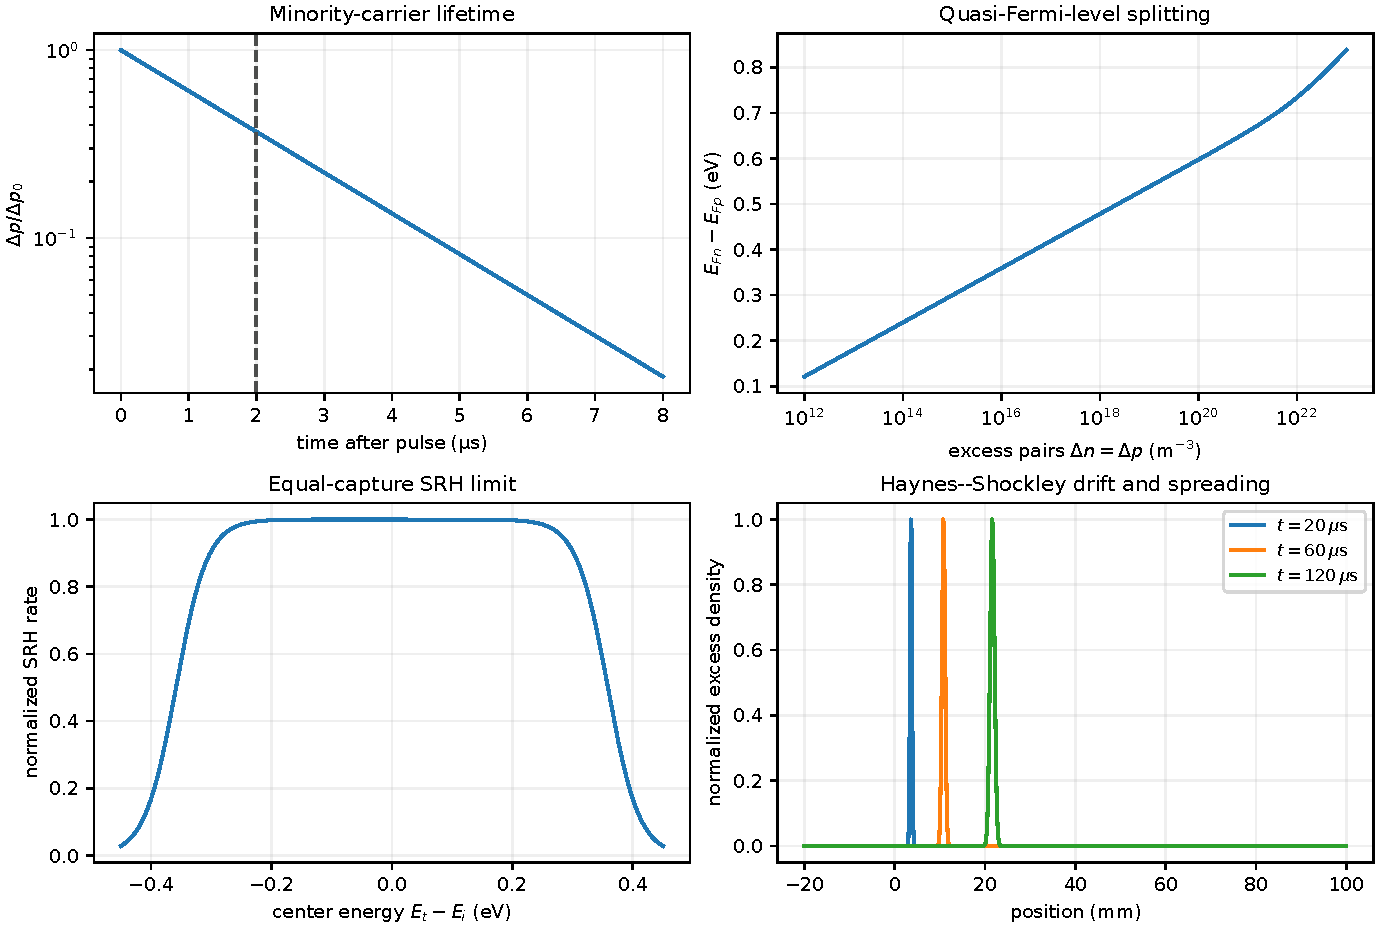
\includegraphics[width=0.94\textwidth]
    {figures/transport-nonequilibrium-carriers.pdf}
  \caption{Temporal lifetime decay, quasi-Fermi-level splitting, the energy
  selectivity of trap-assisted recombination, and the simultaneous drift,
  diffusion, and recombination of a minority-carrier packet.\figurenotebookmark}
  \label{fig:transport-nonequilibrium-carriers}
\end{figure}
\figurenotebooktext{figures/13_generation-recombination-continuity/fig_13_01.ipynb}

\section{Finite-difference continuity and dynamic center kinetics}

The analytic packet in \cref{eq:haynes-shockley-solution} supplies a numerical
oracle, but arbitrary generation profiles, nonlinear SRH rates, and surface
recombination require a numerical solution.  Let
$u_i^m=\Delta p(x_i,t_m)$ on a uniform grid with spacing $\Delta x$.  The
centered diffusion stencil is
\begin{equation}
  \left.\frac{\partial^2u}{\partial x^2}\right|_i
  \simeq
  \frac{u_{i-1}-2u_i+u_{i+1}}{\Delta x^2}.
  \label{eq:continuity-centered-diffusion}
\end{equation}
For positive drift velocity, the second-order upwind derivative is
\begin{equation}
  \left.\frac{\partial u}{\partial x}\right|_i
  \simeq
  \frac{3u_i-4u_{i-1}+u_{i-2}}{2\Delta x};
  \label{eq:continuity-upwind-drift}
\end{equation}
the stencil reverses for negative velocity.  Upwinding follows the direction
from which carriers arrive and prevents the instability of a centered
advection stencil at large cell Péclet number.

For the linear lifetime model, the spatial discretization produces
\begin{equation}
  \frac{\dd\bm u}{\dd t}
  =\bm A\bm u+\bm G.
  \label{eq:continuity-semidiscrete-system}
\end{equation}
The theta method advances this system through
\begin{equation}
  \left(\bm I-\theta\Delta t\bm A\right)\bm u^{m+1}
  =\left[\bm I+(1-\theta)\Delta t\bm A\right]\bm u^m
  +\Delta t\bm G.
  \label{eq:continuity-theta-method}
\end{equation}
Crank--Nicolson uses $\theta=1/2$ and is second order in time; backward Euler
uses $\theta=1$ and damps unresolved transients more strongly.  The packet
validation uses periodic boundaries so only discretization error remains.  Its
discrete carrier number must satisfy
\begin{equation}
  \frac{\Delta x\sum_i u_i(t)}{\Delta x\sum_i u_i(0)}
  =e^{-t/\tau_p}
  \label{eq:continuity-discrete-particle-balance}
\end{equation}
when generation is zero.

\subsection{Nonlinear steady SRH boundary-value problem}

For quasineutral pair injection, set
$n=n_0+u$ and $p=p_0+u$.  A spatially varying source produces the nonlinear
steady equation
\begin{equation}
  D_p\frac{\dd^2u}{\dd x^2}+G(x)
  -U_{\mathrm{SRH}}(n_0+u,p_0+u)=0.
  \label{eq:nonlinear-srh-boundary-problem}
\end{equation}
At an exposed left surface and an ideal collecting right contact, use
\begin{equation}
  D_pu'(0)=Su(0),
  \qquad
  u(L)=0.
  \label{eq:numerical-srh-boundaries}
\end{equation}
The interior finite-difference residual is
\begin{equation}
  F_i=u_{i-1}-2u_i+u_{i+1}
  +\frac{\Delta x^2}{D_p}
  \left[G_i-U_{\mathrm{SRH}}(n_0+u_i,p_0+u_i)\right].
  \label{eq:nonlinear-srh-fd-residual}
\end{equation}
A bounded nonlinear least-squares solve enforces $u_i\ge0$.  The first boundary
row discretizes the Robin condition in \cref{eq:numerical-srh-boundaries}; the
last row fixes the collecting-contact density.  This calculation retains the
full injection dependence of SRH recombination instead of replacing it by one
constant lifetime.

\subsection{Time-dependent center occupation}

The algebraic SRH formula imposes $U_n=U_p$ at every time.  To test that
reduction, integrate the carrier and center equations directly:
\begin{equation}
  \frac{\dd n}{\dd t}=G-U_n,
  \qquad
  \frac{\dd p}{\dd t}=G-U_p,
  \qquad
  N_t\frac{\dd F_t}{\dd t}=U_n-U_p.
  \label{eq:dynamic-center-system}
\end{equation}
Capture and emission can be much faster than carrier decay, so the system is
stiff.  A backward-differentiation-formula solver resolves both time scales.
For the acceptor-like charge convention, the exact invariant
\begin{equation}
  p-n-N_tF_t=\text{constant}
  \label{eq:dynamic-center-charge-invariant}
\end{equation}
provides a stronger diagnostic than solver success alone.

\begin{center}
\small
\begin{tabular}{@{}lll@{}}
\toprule
Numerical check & Result & Acceptance condition \\
\midrule
Packet relative $L_2$ error & $4.999\times10^{-3}$ & below $10^{-2}$ \\
Integrated packet ratio at $40\ \mu\mathrm{s}$ & $0.6065297$ & agrees with $e^{-1/2}$ \\
Nonlinear SRH residual & $8.41\times10^{-10}$ & below $2\times10^{-6}$ \\
Charge-invariant drift & $2.32\times10^{-12}$ & below $10^{-9}$ \\
\bottomrule
\end{tabular}
\end{center}

\begin{figure}[htbp]
  \centering
  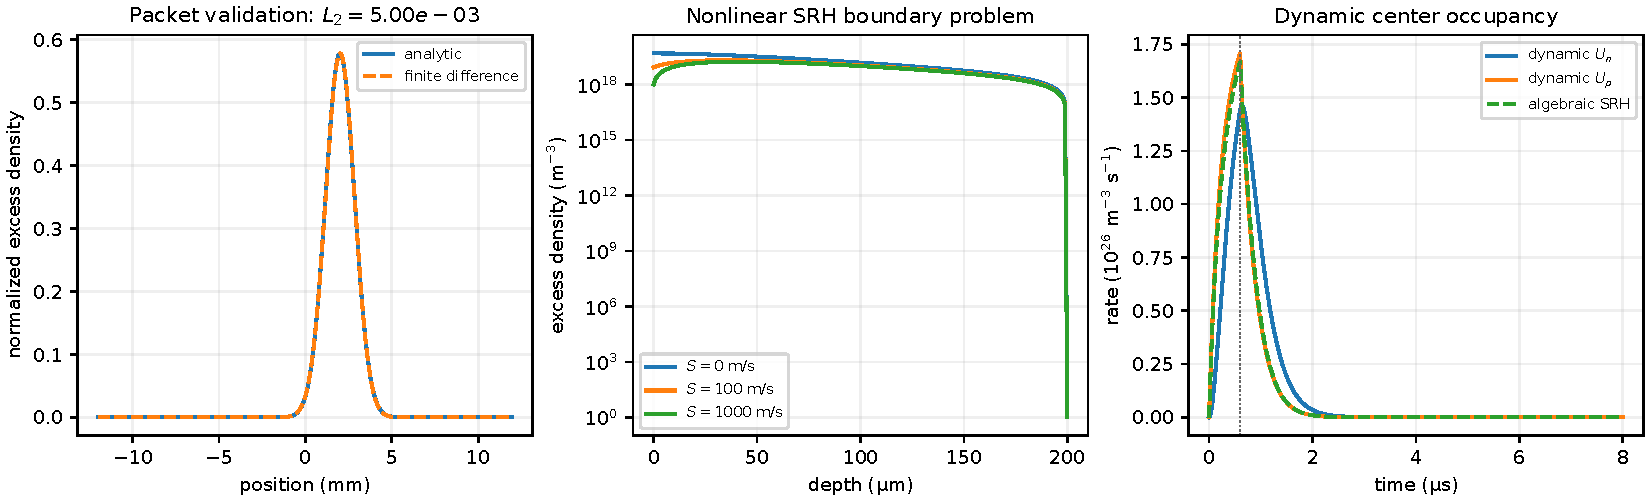
\includegraphics[width=\textwidth]
    {figures/transport-continuity-numerics.pdf}
  \caption{Finite-difference validation against a drifting, diffusing, and
  recombining analytic packet; a nonlinear SRH profile with optical generation
  and surface recombination; and dynamic center rates compared with the
  steady-occupancy SRH reduction.\figurenotebookmark}
  \label{fig:transport-continuity-numerics}
\end{figure}
\figurenotebooktext{figures/13_generation-recombination-continuity/fig_13_01.ipynb}

\section{Range of validity}

A constant lifetime represents the low-injection linearization of one dominant
channel.  The full SRH rate requires the center energy, degeneracy, density,
capture cross sections, and charge state.  Its algebraic form assumes steady
center occupancy and negligible stored center charge; otherwise the occupancy
requires an additional rate equation.  Several center levels contribute
separate rates.  Auger recombination replaces the lifetime law at high carrier
density, while depleted regions exhibit net SRH generation.  Quasi-Fermi
levels require each carrier population to remain internally thermalized.
Diffusion-length solutions assume uniform coefficients and neutral regions;
depletion fields and spatially varying material parameters require the coupled
drift--diffusion--Poisson system.

\section{Chapter summary}

Generation displaces carrier populations from $np=n_i^2$, and recombination
restores equilibrium.  Low-level excess carriers decay with a lifetime and over
a diffusion length.  Direct, recombination-center-assisted, and Auger channels
produce distinct density dependences; the SRH channel reverses sign to generate
carriers in depleted material.  Quasi-Fermi levels quantify nonequilibrium
carrier populations.  Continuity combines these local rates with carrier
current, while a moving minority-carrier packet exposes mobility, diffusivity,
and lifetime separately.
